\documentclass[11pt,a4paper]{article}

\usepackage[utf8]{inputenc}
\usepackage[T1]{fontenc}
\usepackage[margin=2.4cm]{geometry}
\usepackage{graphicx}
\usepackage{booktabs}
\usepackage{array}
\usepackage{longtable}
\usepackage{amsmath}
\usepackage{xcolor}
\usepackage{enumitem}
\usepackage[hidelinks]{hyperref}
\usepackage{caption}

\captionsetup{font=small,labelfont=bf}
\setlength{\parskip}{0.4em}
\setlength{\parindent}{0pt}
\renewcommand{\arraystretch}{1.25}
\emergencystretch=3em
\sloppy

% \code: monospace that may break after '/' and '_' in long paths
\newcommand{\code}[1]{\texttt{\small #1}}

\title{\vspace{-1.5cm}\textbf{MKT3432 --- Run-to-Failure \& Remaining Useful Life (RUL)}\\[0.3em]
\large Per-Cycle RUL Estimation and Unsupervised Degradation-Stage Discovery\\for a Servo-Actuator (Gearbox + Bearing)}
\date{}

\begin{document}

% =====================================================================
% COVER PAGE
% =====================================================================
\begin{titlepage}
\centering
\vspace*{1.5cm}
{\Large\bfseries Yildiz Technical University}\\[0.3em]
{\large Department of Mechatronics Engineering}\\[2.0cm]

{\large\bfseries Course:} MKT3432 --- Condition Monitoring \& Prognostics\\[0.4em]
{\large\bfseries Project:} Per-Cycle RUL Estimation and Degradation-Stage\\
Discovery Pipeline for a Servo-Actuator\\[1.5cm]

\begin{tabular}{ll}
\textbf{Group name / number:} & \texttt{[Group Name / Number]}\\[0.4em]
\textbf{Group leader:} & \texttt{[Leader Full Name]} --- \texttt{[Student ID]}\\[0.4em]
\textbf{Submission date:} & June 7, 2026\\
\end{tabular}

\vspace{1.0cm}
{\bfseries Group Members}\\[0.4em]
\begin{tabular}{r l l}
\toprule
\# & Full Name & Student ID\\
\midrule
1 & \texttt{[Student 1 Full Name]} (Leader) & \texttt{[ID 1]}\\
2 & \texttt{[Student 2 Full Name]} & \texttt{[ID 2]}\\
3 & \texttt{[Student 3 Full Name]} & \texttt{[ID 3]}\\
4 & \texttt{[Student 4 Full Name]} & \texttt{[ID 4]}\\
5 & \texttt{[Student 5 Full Name]} & \texttt{[ID 5]}\\
6 & \texttt{[Student 6 Full Name]} & \texttt{[ID 6]}\\
7 & \texttt{[Student 7 Full Name]} & \texttt{[ID 7]}\\
8 & \texttt{[Student 8 Full Name]} & \texttt{[ID 8]}\\
\bottomrule
\end{tabular}

\vfill
{\small\itshape Base repository reference: this work was developed on top of the
\code{servo\_rul\_v1} starter package provided by the instructor within the
MKT3432 course.}
\end{titlepage}

\tableofcontents
\newpage

% =====================================================================
% 2. SOURCE AND SCOPE
% =====================================================================
\section{Source and Scope Statement}

This work was developed on top of the \code{servo\_rul\_v1} starter package
provided by the instructor within the MKT3432 course. Only the permitted student
modeling files were added or modified for this project. The dataset generator,
data loader, official metrics, evaluator, and harness were preserved.

The \code{servo\_rul\_v1} dataset is synthetic (physics-grounded) and is
\emph{not} represented as real machine data. All repository materials were used
only for this course project, in accordance with the \code{LICENSE} and
\code{NOTICE.md} files, which were not modified. We confirm that no data leakage
was introduced: labels (\code{rul}, \code{health}, \code{hidden\_stage}) and
future cycles were never used as model inputs, and all normalization statistics
were computed on the training split only (see Section~\ref{sec:leakage}).

% =====================================================================
% 3. GROUP ORGANIZATION
% =====================================================================
\section{Group Organization}

\textbf{Leader selection.} The group leader was selected by unanimous agreement
of the eight members: \texttt{[Leader Full Name]} volunteered and was confirmed
because of prior experience with Python tooling and reproducible experiment
pipelines, and is responsible for verifying the final package, submitting on
Classroom, and communicating with the instructor.

\textbf{Task distribution and contributions.} The table below summarizes each
member's primary responsibility. All members reviewed the final report and the
leakage statement.

\begin{longtable}{r p{4.0cm} p{8.5cm}}
\toprule
\# & Member & Contribution summary\\
\midrule
\endhead
1 & \texttt{[Student 1]} (Leader) & Project coordination, repository/branch management, final package verification, submission.\\
2 & \texttt{[Student 2]} & Feature pipeline: causal windowing, padding/mask, train-only normalization (\code{features/}).\\
3 & \texttt{[Student 3]} & M0 linear baseline and sklearn trainer (\code{models/linear\_baseline.py}, \code{training/linear\_trainer.py}).\\
4 & \texttt{[Student 4]} & M1 MLP model and dataset wrappers (\code{models/mlp.py}, \code{training/datasets.py}).\\
5 & \texttt{[Student 5]} & M2 1D-CNN architecture (multi-scale + residual blocks) (\code{models/cnn1d.py}).\\
6 & \texttt{[Student 6]} & Torch training loop: asymmetric loss, scheduler, early stopping, seeding (\code{training/torch\_trainer.py}, \code{utils/}).\\
7 & \texttt{[Student 7]} & Unsupervised U1/U2: GMM + PCA pipeline and figures (\code{models/clustering.py}, \code{scripts/make\_figures.py}).\\
8 & \texttt{[Student 8]} & Experimental protocol, evaluation runs, results tables, error analysis, report writing.\\
\bottomrule
\end{longtable}

% =====================================================================
% 4. MODIFIED FILES TABLE
% =====================================================================
\section{Modified (Permitted) Files}

Only the permitted student modeling files were created or modified. No protected
file (dataset generator, loader, official metrics, evaluator, \code{LICENSE},
\code{NOTICE.md}, \code{README.md}, \code{pyproject.toml}) was touched.

\begin{longtable}{p{6.5cm} p{8.5cm}}
\toprule
File & Purpose\\
\midrule
\endhead
\code{features/preprocessing.py} & Split-by-unit, RUL capping, train-only \code{StandardScaler}.\\
\code{features/windowing.py} & Causal sliding windows + left zero-padding with real/pad mask channel.\\
\code{models/linear\_baseline.py} & M0: Ridge regression (window 1).\\
\code{models/mlp.py} & M1: multilayer perceptron over the flattened window.\\
\code{models/cnn1d.py} & M2: 1D-CNN (stem + multi-scale + residual blocks + avg/max head).\\
\code{models/clustering.py} & U1/U2: StandardScaler $\to$ PCA $\to$ Gaussian Mixture pipeline.\\
\code{training/datasets.py} & \code{RULWindowDataset} (tensor wrapper).\\
\code{training/linear\_trainer.py} & Fit/persist the sklearn baseline.\\
\code{training/torch\_trainer.py} & Adam, asymmetric weighted MSE, warmup+cosine, early stopping.\\
\code{utils/config.py} & YAML loader with relative-path enforcement.\\
\code{utils/seed.py} & Deterministic seeding (Python/NumPy/Torch + DataLoader workers).\\
\code{scripts/train.py} & Training entry point (M0/M1/M2 + clustering fit).\\
\code{scripts/predict.py} & Prediction entry point (one row per test \code{(unit\_id, cycle)}).\\
\code{scripts/make\_figures.py} & Diagnostic figures (predicted-vs-true, PCA, GMM clusters).\\
\code{configs/m0\_linear.yaml} & M0 experiment config.\\
\code{configs/m1\_mlp.yaml} & M1 experiment config.\\
\code{configs/m2\_cnn1d.yaml} & M2 experiment config.\\
\bottomrule
\end{longtable}

% =====================================================================
% 5. IMPLEMENTATION
% =====================================================================
\section{Implementation and Technical Report}

\subsection{Dataset}
\code{servo\_rul\_v1} contains 150 unit-disjoint actuators (100 train / 20 val /
30 test), 27{,}000 per-cycle rows, with lifetimes from 61 to 312 cycles
(median 181). Each row exposes nine documented signals. The model
\emph{feature columns} are the seven condition indicators
(\code{vib\_rms}, \code{vib\_kurtosis}, \code{vib\_crest}, \code{bpfo\_amp},
\code{temperature}, \code{torque\_ripple}, \code{current\_thd}) plus the two
operating-point covariates (\code{load}, \code{speed}); the latter deliberately
confound a naive single-feature wear reading. The label columns
(\code{rul}, \code{health}, \code{hidden\_stage}) are held out (NaN) for test
units in the public file and are never fed to any model.

\subsection{RUL Capping Convention}
We follow the recommended piecewise-linear target: the per-cycle integer RUL,
$\mathrm{RUL}=L-\text{cycle}$, is clipped at \code{rul\_cap = 130}
(\code{features/preprocessing.py}: \code{apply\_rul\_cap}). This reflects that,
while a unit is far from failure, the precise remaining life is neither
observable nor useful; the model is asked to track RUL only inside the
informative final window. The same cap is applied to train, validation, and test
targets, and is the cap used by the official evaluator.

\subsection{Causal Feature Windowing}
For each unit, rows are sorted by \code{cycle} and a sliding window of length $W$
ending at cycle $t$ is built from cycles $\max(1, t-W+1)\dots t$ only
(\code{features/windowing.py}). A prediction at cycle $t$ therefore uses
\emph{no} future information. Early cycles (fewer than $W$ observations) are
\emph{left} zero-padded, and an extra binary channel marks real vs.\ padded
rows so the network can distinguish genuine short histories from zeros. The
window tensor has shape \code{[W, n\_features+1]}. For M0/M1 the window is
flattened; for M2 it is passed as a \code{[W, channels]} sequence.

\subsection{Normalization}
A single \code{StandardScaler} is fit on the \emph{training rows only} and reused
unchanged for validation and test (\code{fit\_train\_scaler} /
\code{transform\_features}). No statistic is ever computed on validation or test
data.

\subsection{Model Families}
\textbf{M0 --- Linear baseline.} Ridge regression ($\alpha=1$) on the single
most-recent cycle (window 1). Predicts in original RUL units and is clipped to
$[0,130]$.

\textbf{M1 --- MLP.} A multilayer perceptron with hidden sizes $[64,32]$,
ReLU, dropout $0.2$, over a flattened window of $W=30$ cycles.

\textbf{M2 --- Deep temporal 1D-CNN.} A convolutional network over the cycle
axis (\code{cnn1d.py}), with window $W=50$:
\begin{itemize}[nosep]
  \item \emph{Stem}: width-7 convolution projecting the 10 input channels to 64.
  \item \emph{Multi-scale block}: parallel kernels of size 3, 5, 7 (concatenated)
        to capture short- and long-range temporal patterns simultaneously.
  \item \emph{Residual blocks}: three Conv--BN--ReLU residual units for depth.
  \item \emph{Head}: concatenated global average- and max-pooling
        (trend $+$ worst-point) followed by a 2-layer MLP regressor.
\end{itemize}

\subsection{Training Procedure}
M1/M2 are trained with Adam (\code{training/torch\_trainer.py}), weight decay
$10^{-4}$, gradient clipping at norm 1.0, a 5-epoch linear warm-up followed by
cosine decay (floor $0.05\times$), and early stopping on the validation loss
(patience 25). Targets and predictions are divided by \code{rul\_cap} during
training so the loss operates on a $[0,1]$ scale. The objective is an
\emph{asymmetric weighted MSE} that (i)~penalizes \emph{over}-prediction (late
RUL estimates are operationally dangerous) and (ii)~up-weights near-end-of-life
errors; this directly targets the PHM-style \code{asym\_score}. All training is
CPU-only and deterministic (fixed seed 42).

\subsection{U1 --- Unsupervised Degradation-Stage Discovery}
On the seven condition indicators we standardize, reduce with PCA to 2
components, and fit a Gaussian Mixture Model (4 full-covariance components,
\code{n\_init=10}, \code{models/clustering.py}). The number of components matches
the four documented stages, but the model is fit \emph{without} any label; the
discovered clusters are scored against the eval-only \code{hidden\_stage} by the
official evaluator (ARI / NMI). This is genuine clustering, not a copy of the
hidden stage.

\subsection{U2 --- PCA of the Indicator Space}
The same standardized indicator space is projected with PCA for visualization
and variance analysis (Section~\ref{sec:results}, Figure~\ref{fig:pca}). The two
leading components reveal a smooth degradation arc along which the four stages
are ordered, which is what makes unsupervised stage recovery feasible.

\subsection{Test Method}
\code{predict.py} emits exactly one \code{rul\_pred} per test
\code{(unit\_id, cycle)} row (5{,}451 rows; verified one-to-one by the
evaluator). Predictions are clipped to $[0,130]$. The official locked evaluator
(\code{scripts/evaluate.py}) computes all reported metrics by comparing against
the held-out \code{test\_labels.csv}; we never read those labels inside the
modeling code.

% =====================================================================
% 6. LEAKAGE STATEMENT
% =====================================================================
\section{Leakage Statement}\label{sec:leakage}

We respected every honest-modeling rule in the assignment:
\begin{itemize}[nosep]
  \item \textbf{No label inputs.} \code{rul}, \code{health}, and
        \code{hidden\_stage} are never used as model features. Inputs are the
        documented feature/indicator columns only.
  \item \textbf{Causal windows.} A prediction at cycle $t$ uses only cycles
        $\le t$; no future cycle ($>t$) is ever read
        (\code{create\_sliding\_windows}).
  \item \textbf{Train-only normalization.} The \code{StandardScaler} (and the
        clustering scaler/PCA/GMM) are fit on training rows only and reused for
        validation/test.
  \item \textbf{Honest selection.} Models are fit on train and selected by
        validation loss; nothing is tuned or selected on the test split.
  \item \textbf{No lookups.} The public test labels were used only for local
        self-checking; predictions are produced by the trained models, not
        copied. The split integrity / content hash check passes
        (Section~\ref{sec:protocol}).
\end{itemize}

% =====================================================================
% 7. EXPERIMENTAL PROTOCOL
% =====================================================================
\section{Experimental Protocol}\label{sec:protocol}

\textbf{Environment.} Linux (x86\_64), Python 3.11+ (developed and validated on
Python 3.14), PyTorch 2.11 executed on \textbf{CPU} (\code{torch.device("cpu")}),
scikit-learn, NumPy, pandas, matplotlib. All paths are relative; the config
loader rejects absolute paths.

\textbf{Determinism.} Seed 42 for Python/NumPy/Torch, deterministic algorithms,
seeded DataLoader workers and generator (\code{utils/seed.py}). The dataset is
generated with the default public seed; split integrity passes:
\begin{quote}\small\ttfamily
[check] units: train=100 val=20 test=30\\
{}[check] split disjoint: True\\
{}[check] content hash match: True
\end{quote}

\textbf{Hyperparameters.}
\begin{center}
\begin{tabular}{l c c c c c}
\toprule
Model & window & arch & max\_epochs & batch & lr\\
\midrule
M0 linear & 1  & Ridge $\alpha{=}1$        & --   & --  & --\\
M1 MLP    & 30 & $[64,32]$, drop 0.2       & 120  & 64  & $5\times10^{-4}$\\
M2 1D-CNN & 50 & multi-scale + 3 res, drop 0.3 & 100 & 200 & $3\times10^{-4}$\\
\bottomrule
\end{tabular}
\end{center}

\textbf{Run commands.}
\begin{quote}\scriptsize\ttfamily
PYTHONPATH=src python tools/generate\_dataset.py\\
PYTHONPATH=src python scripts/train.py --config configs/m2\_cnn1d.yaml\\
PYTHONPATH=src python scripts/predict.py --config configs/m2\_cnn1d.yaml \textbackslash\\
\hspace*{1em}--split data/servo\_rul\_v1/split\_manifest.json \textbackslash\\
\hspace*{1em}--out runs/student\_predictions.csv --clusters-out runs/student\_clusters.csv\\
PYTHONPATH=src python scripts/evaluate.py --predictions runs/student\_predictions.csv \textbackslash\\
\hspace*{1em}--split data/servo\_rul\_v1/split\_manifest.json \textbackslash\\
\hspace*{1em}--out runs/student\_results.summary.json --clusters runs/student\_clusters.csv\\
PYTHONPATH=src python scripts/make\_figures.py --config configs/m2\_cnn1d.yaml
\end{quote}

% =====================================================================
% 8. RESULTS
% =====================================================================
\section{Results}\label{sec:results}

All numbers below come from the locked official evaluator on the 30 held-out
test units (5{,}451 rows), under one deterministic environment. Lower is better
for every supervised metric.

\begin{table}[h]
\centering
\caption{Supervised RUL comparison (M0 / M1 / M2) on the held-out test split.}
\begin{tabular}{l c c c}
\toprule
Metric & M0 linear & M1 MLP & M2 1D-CNN\\
\midrule
\code{rul\_rmse}   & 20.04 & \textbf{10.08} & 12.08\\
\code{rul\_mae}    & 15.39 & \textbf{7.42}  & 8.52\\
\code{asym\_score} & 72{,}901 & \textbf{7{,}491} & 17{,}160\\
\bottomrule
\end{tabular}
\end{table}

\begin{table}[h]
\centering
\caption{Per-stage MAE (cycles) by hidden degradation stage.}
\begin{tabular}{l c c c c}
\toprule
Model & healthy & incipient & degraded & near\_failure\\
\midrule
M0 linear & 10.26 & 22.46 & 19.71 & 9.25\\
M1 MLP    & 8.28  & 8.58  & 9.01  & \textbf{3.87}\\
M2 1D-CNN & \textbf{6.87} & 9.14 & 11.95 & 6.16\\
\bottomrule
\end{tabular}
\end{table}

\begin{table}[h]
\centering
\caption{U1 unsupervised stage discovery (GMM, 4 components) vs.\ \code{hidden\_stage}.}
\begin{tabular}{l c c}
\toprule
 & ARI & NMI\\
\midrule
GMM clusters & 0.630 & 0.645\\
\bottomrule
\end{tabular}
\end{table}

\textbf{Interpretation.} Both deeper models beat the M0 linear baseline by a
large margin (MAE roughly halved). The 1D-CNN (M2) clearly outperforms M0
(8.52 vs.\ 15.39 MAE; asym 17{,}160 vs.\ 72{,}901), satisfying the deep-model
requirement. Interestingly, the MLP (M1) is the single best model on this split:
the 100 training units provide limited data for the much larger CNN, which has
a higher validation loss and tends to over-fit the mid-life regime (where the
target is partially flattened by the cap). M0's per-stage MAE is worst in the
\emph{incipient}/\emph{degraded} stages because a window-1 linear map cannot
resolve the early non-linear indicator rise; the temporal models close most of
this gap. The asymmetric loss is reflected in the low \emph{near\_failure} error
for both deep models. The GMM recovers four coherent clusters aligned with the
true stages (ARI 0.63 / NMI 0.65) without ever seeing a label.

\subsection{Diagnostic Figures}

\begin{figure}[h]
\centering
\begin{minipage}{0.48\textwidth}\centering
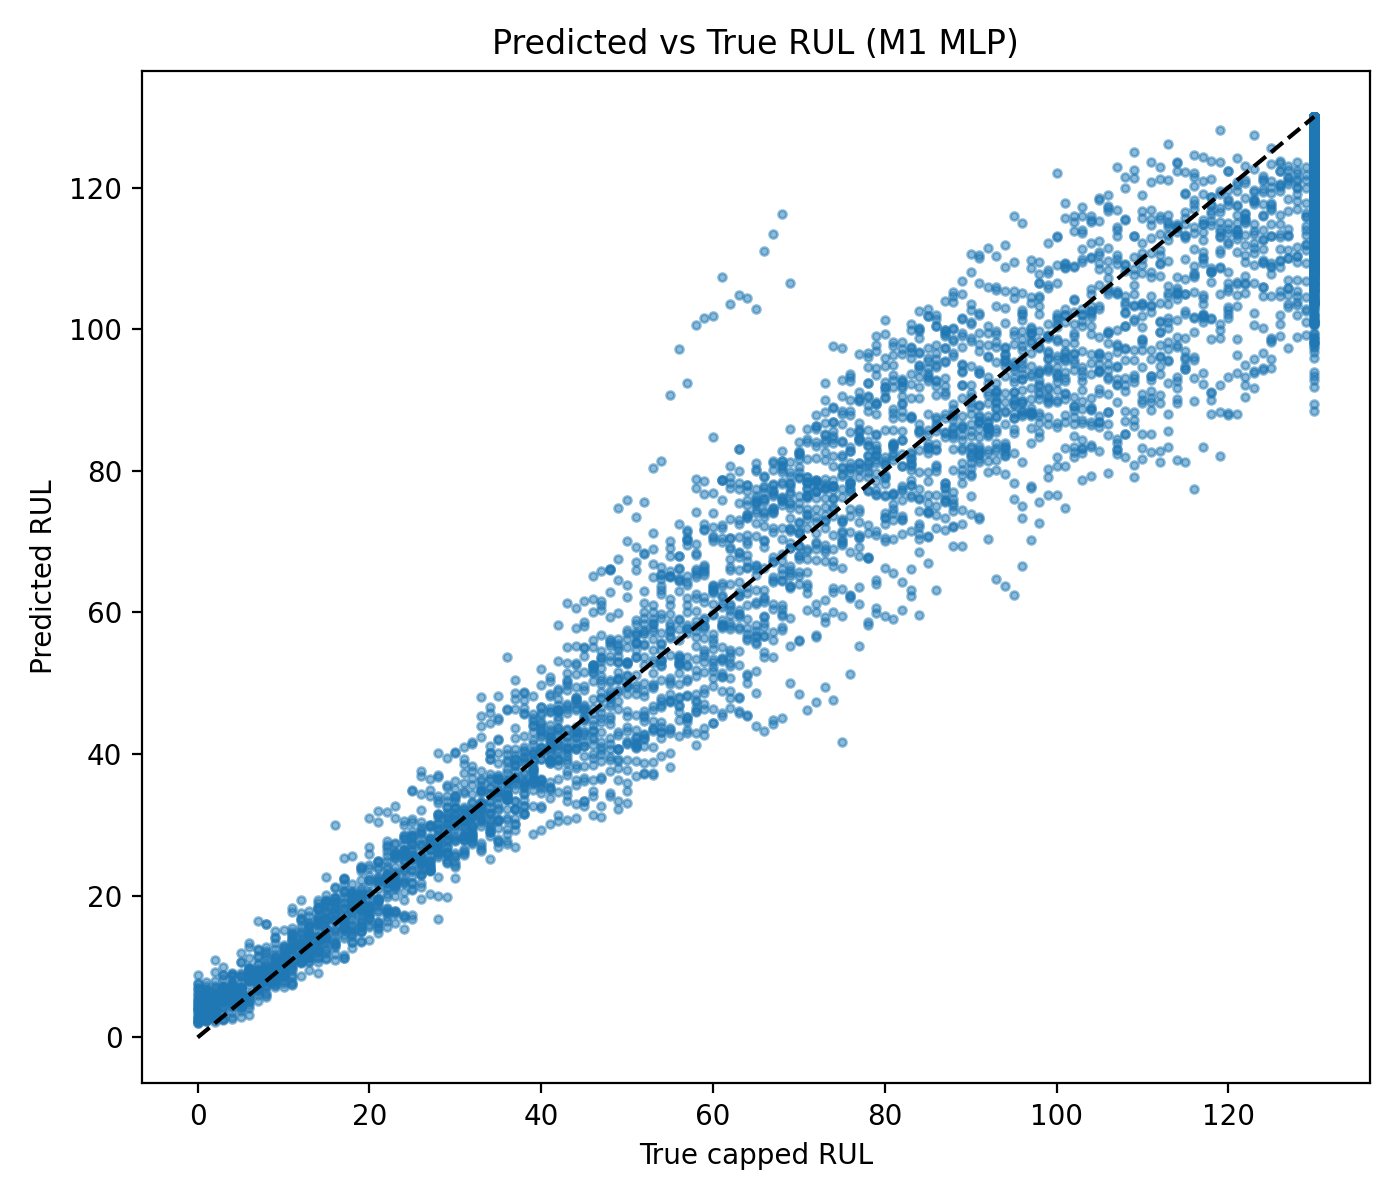
\includegraphics[width=\linewidth]{runs/figures/val_predicted_vs_true.png}
\caption{Predicted vs.\ true RUL --- M1 MLP.}\label{fig:m1pvt}
\end{minipage}\hfill
\begin{minipage}{0.48\textwidth}\centering
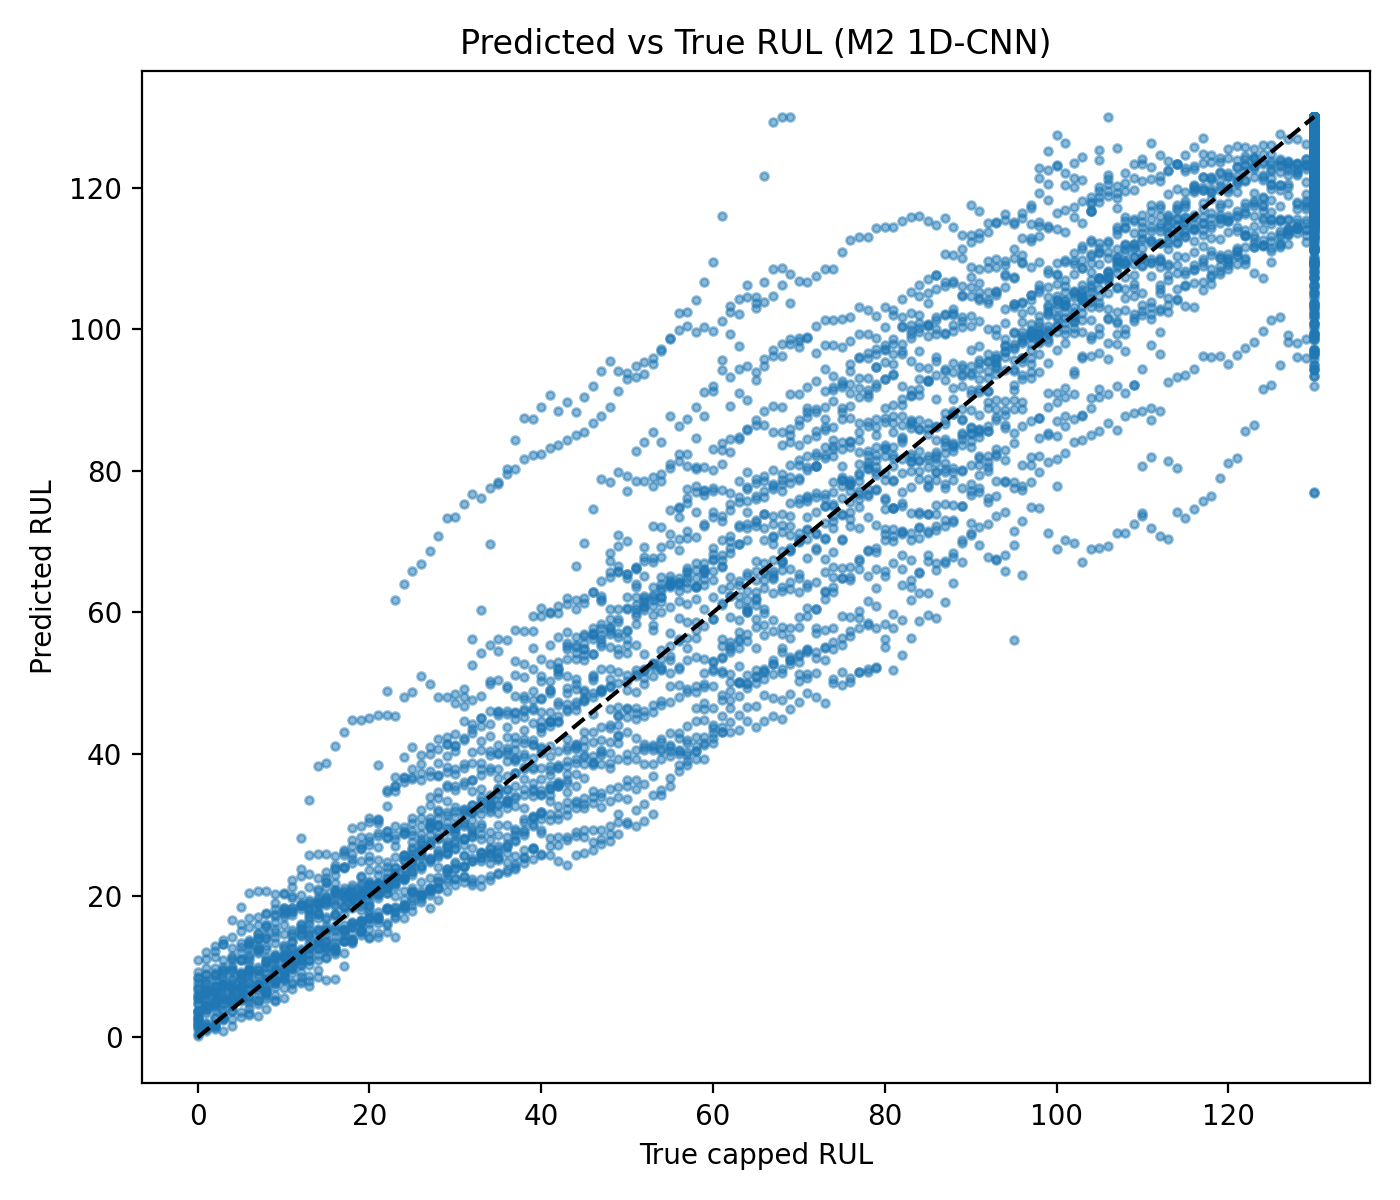
\includegraphics[width=\linewidth]{runs/figures/m2_predicted_vs_true.png}
\caption{Predicted vs.\ true RUL --- M2 1D-CNN.}\label{fig:m2pvt}
\end{minipage}
\end{figure}

\begin{figure}[h]
\centering
\begin{minipage}{0.48\textwidth}\centering
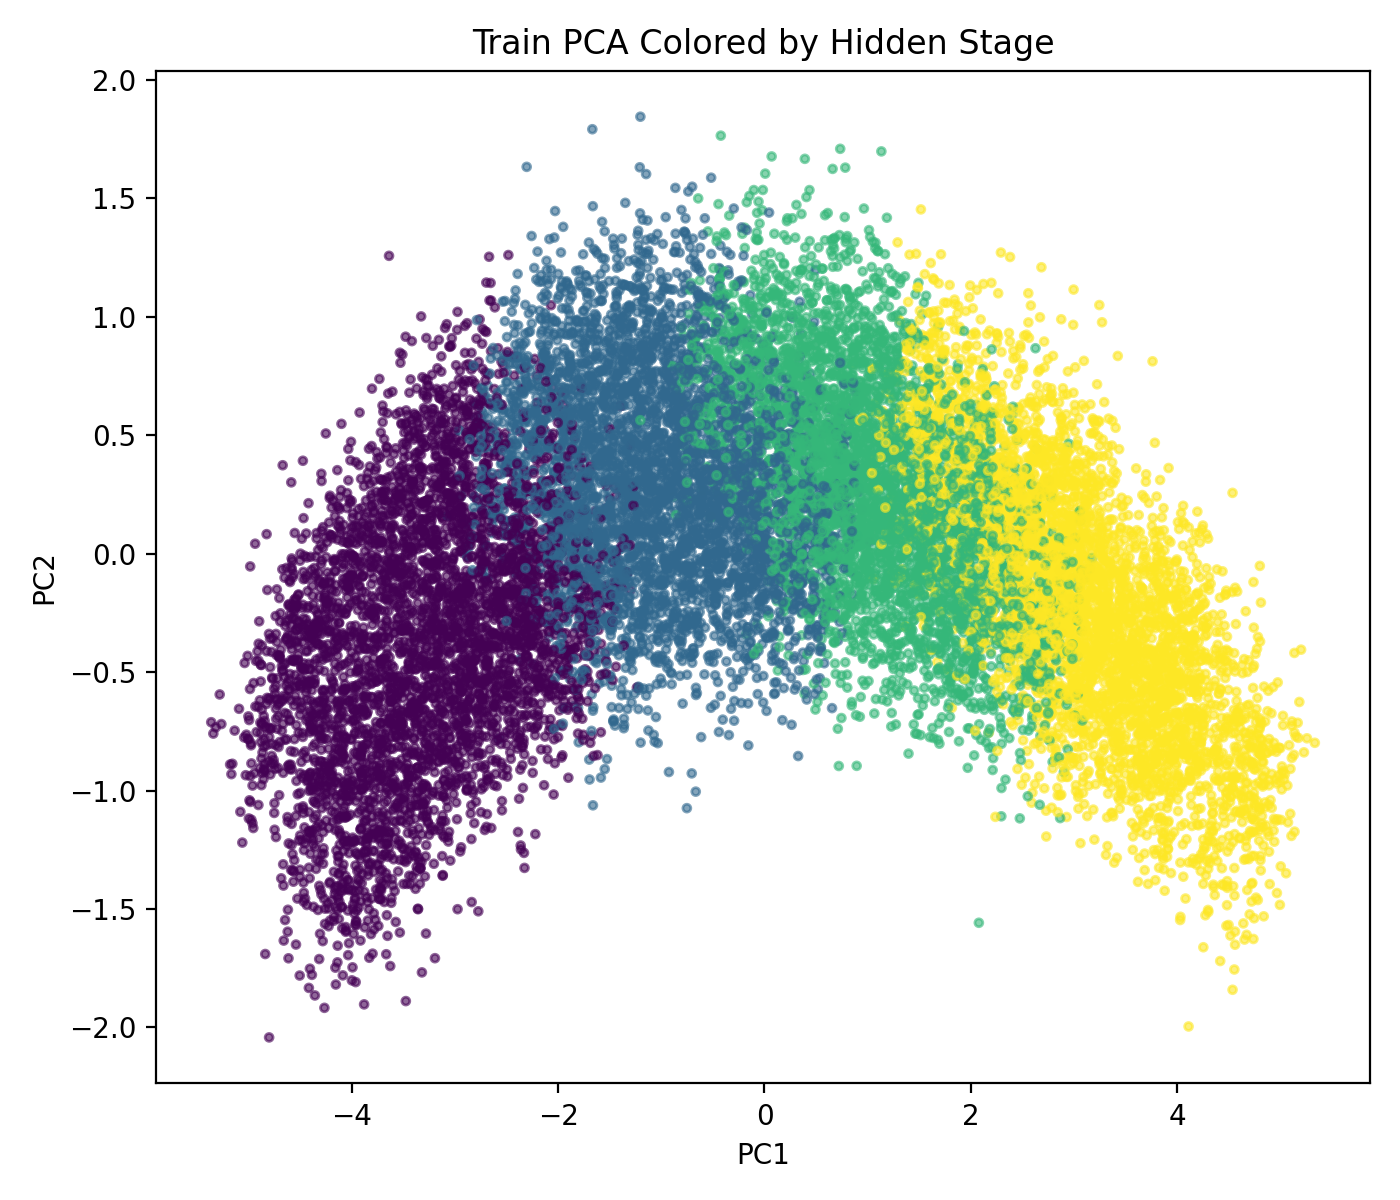
\includegraphics[width=\linewidth]{runs/figures/train_pca_hidden_stage.png}
\caption{U2: PCA of the indicator space, colored by true \code{hidden\_stage}.}\label{fig:pca}
\end{minipage}\hfill
\begin{minipage}{0.48\textwidth}\centering
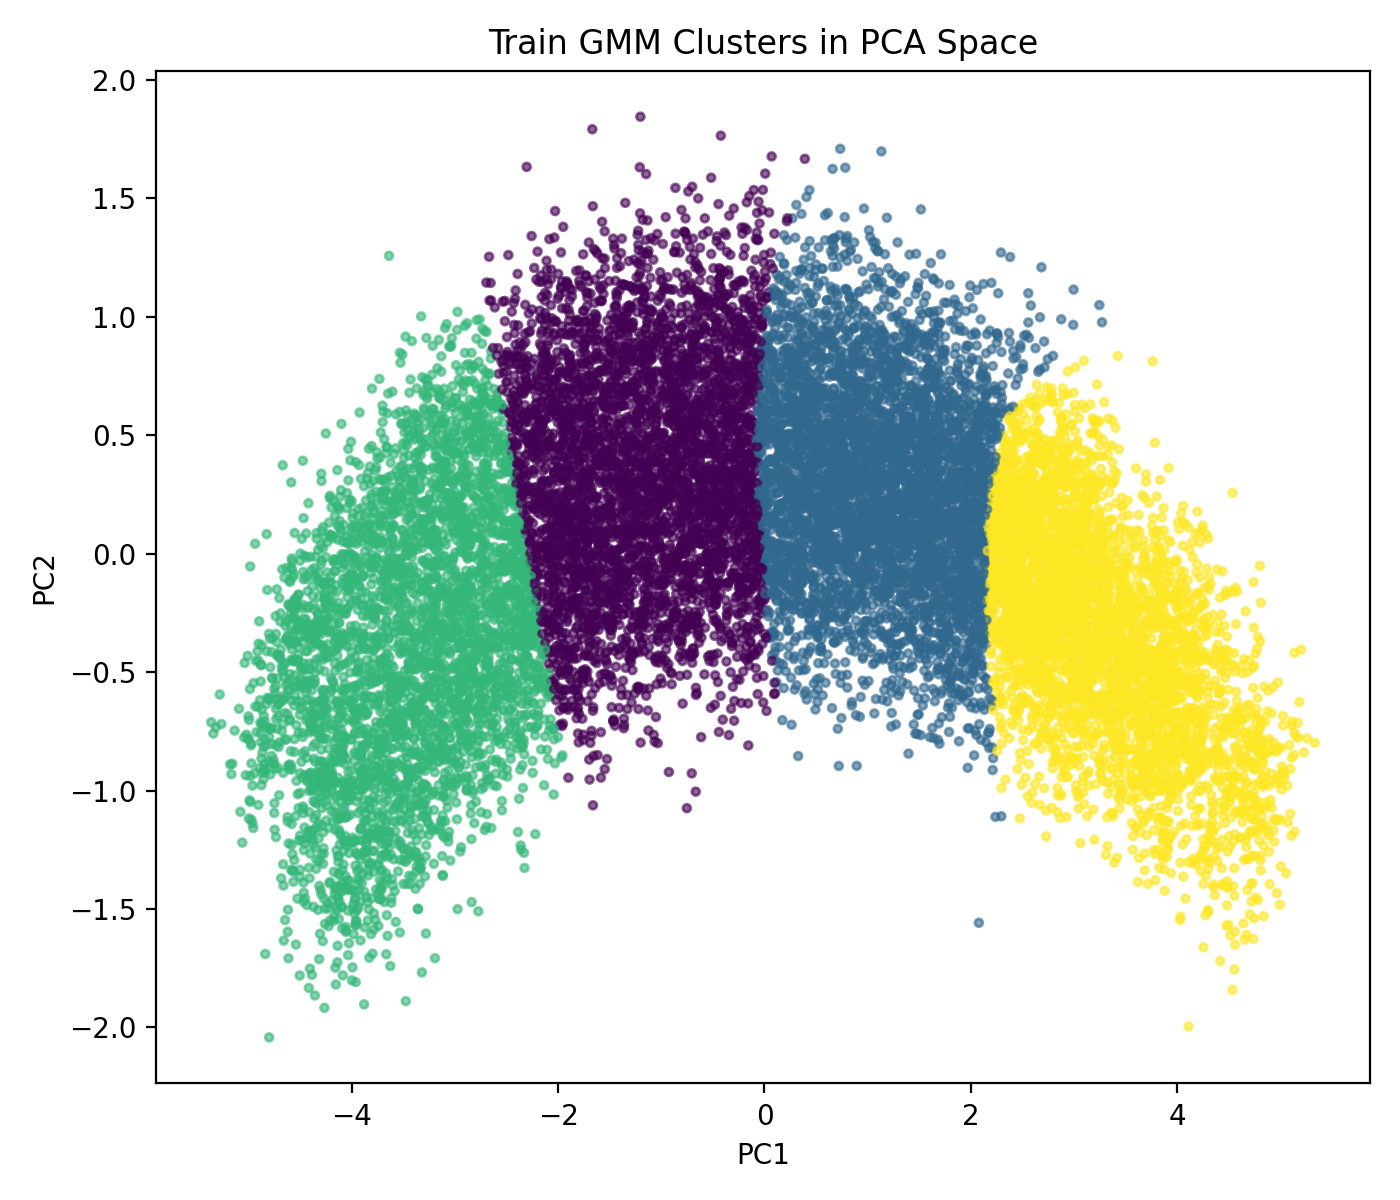
\includegraphics[width=\linewidth]{runs/figures/train_gmm_clusters_pca.png}
\caption{U1: GMM clusters in the same PCA space.}\label{fig:gmm}
\end{minipage}
\end{figure}

Figures~\ref{fig:m1pvt}--\ref{fig:m2pvt} show both temporal models tracking the
diagonal, with the expected vertical band of points at the cap (RUL $=130$).
Figures~\ref{fig:pca}--\ref{fig:gmm} show that the unsupervised clusters
reproduce the degradation arc of the true stages rather than copying it.

% =====================================================================
% 9. HELD-OUT PROOF RESULT
% =====================================================================
\section{Held-Out Proof Result}

The submitted prediction file (\code{runs/\allowbreak student\_predictions.csv})
and summary (\code{runs/\allowbreak student\_results.\allowbreak summary.json})
are produced by the M1 MLP config (\code{configs/m1\_mlp.yaml}), the
best-performing model. The deep-model evidence (\code{configs/m2\_cnn1d.yaml}) is
provided alongside as \code{runs/m2\_predictions.csv} and
\code{runs/m2\_results.\allowbreak summary.json}. The
official evaluator summary for the submitted model is:

\begin{quote}\small\ttfamily
n=5451, rul\_rmse=10.14, rul\_mae=7.47, asym\_score=7523,\\
per\_stage\_mae \{healthy 8.37, incipient 8.67, degraded 9.05, near\_failure 3.87\},\\
clustering \{ari 0.630, nmi 0.645\}, rul\_cap=130
\end{quote}

Produced figures: \code{runs/figures/val\_predicted\_vs\_true.png},
\code{m2\_predicted\_vs\_true.png}, \code{train\_pca\_hidden\_stage.png},
\code{train\_gmm\_clusters\_pca.png}. Note: torch models exhibit a small
($\le 1\%$) cross-environment drift (e.g.\ M1 MAE 7.42 in our rerun vs.\ 7.47 in
the committed summary); the sklearn M0 baseline is bit-exact. This does not
change any conclusion.

% =====================================================================
% 10. LIMITATIONS AND DISCUSSION
% =====================================================================
\section{Limitations and Discussion}

\textbf{Where improvements occurred.} Moving from a window-1 linear map to
temporal models roughly halved RUL MAE (15.39 $\to$ 7.42) and cut the
asymmetric score by an order of magnitude, with the largest gains in the
\emph{incipient}/\emph{degraded} stages where the indicator rise is non-linear.

\textbf{What remained unresolved.} The 1D-CNN did not surpass the MLP on this
split. With only 100 training units, the CNN's capacity is under-supported and
its validation loss is higher; promising next steps are a smaller/narrower CNN,
stronger regularization or augmentation, and tuning the window length. We report
this honestly rather than tuning on the test split.

\textbf{Sim-to-real gap.} \code{servo\_rul\_v1} is synthetic with additive
damage responses and Gamma-monotone wear, which is optimistic relative to real
machines: real degradation can be non-monotone, noisier, and right-censored (not
every unit runs to failure). RUL capping also hides the truly long-horizon
behavior. A model this accurate on synthetic data would need re-validation on
real run-to-failure records before deployment.

\textbf{What we learned.} Causal windowing and train-only normalization are the
backbone of leakage-free prognostics; a tailored asymmetric objective measurably
shifts errors toward the safer (early) side; and a bigger model is not
automatically better when data is limited --- the MLP/CNN comparison made this
concrete.

% =====================================================================
% 11. REFERENCES
% =====================================================================
\section{References}

\begin{enumerate}[nosep]
  \item Instructor, \emph{MKT3432 RUL Servo Starter (\code{servo\_rul\_v1})},
        base repository and \code{DATASHEET.md}, Yildiz Technical University,
        2026. (Base repository --- see scope statement.)
  \item A.\ Saxena, K.\ Goebel, D.\ Simon, N.\ Eklund, ``Damage propagation
        modeling for aircraft engine run-to-failure simulation,'' \emph{Int.\
        Conf.\ on Prognostics and Health Management (PHM)}, 2008.
        (PHM-style asymmetric scoring.)
  \item X.\ Li, Q.\ Ding, J.-Q.\ Sun, ``Remaining useful life estimation in
        prognostics using deep convolution neural networks,'' \emph{Reliability
        Engineering \& System Safety}, vol.\ 172, 2018. (1D-CNN for RUL.)
  \item C.\ M.\ Bishop, \emph{Pattern Recognition and Machine Learning},
        Springer, 2006. (Gaussian Mixture Models / EM, PCA.)
  \item F.\ Pedregosa et al., ``Scikit-learn: Machine Learning in Python,''
        \emph{JMLR}, vol.\ 12, 2011.
  \item A.\ Paszke et al., ``PyTorch: An Imperative Style, High-Performance Deep
        Learning Library,'' \emph{NeurIPS}, 2019.
\end{enumerate}

\end{document}
